\section{Comparing Transfers via Intermediate Sun-Earth Halos to Direct Transfers}
Just like the example tradespace provided in Section 4.3.3, with \cref{fig:tradespace}, for a given
cislunar departure orbit, the "direct" transfers are compared to those that stage in an
intermediate Sun-Earth unstable halo orbit. Tradespaces for all of the departure orbits used in
this investigation are provided in Appendix A, but a few will be introduced in this section to
better facilitate the comparison.

In all of the cases examined in this investigation, the family of "direct" transfers overall has
lower times-of-flight than the staging transfers. As an example, in \cref{fig:tradespace}, the blue
points representing the "direct" transfers mostly lie to the left of the red transfers that utilize
a staging orbit. The transfers with the lowest times-of-flight generally have much higher
$\Delta v$ costs, but there are some cases where the $\Delta v$ lies below the baseline of the
"Hohmann" transfer.

\subsection{Cost Function}
In the example of \cref{fig:tradespace}, the "direct" transfer family also contains the
minimum-$\Delta v$ solutions, which also have lower times-of-flight than the staging orbit
transfers. However, this is not always the case, as shown in \cref{fig:lowDeltav}. As a result,
often a choice needs to be made balancing TOF and maneuver $\Delta v$ cost. A cost function can
help select desirable transfers that balance these two parameters.

\begin{figure}[ht]
    \centering
    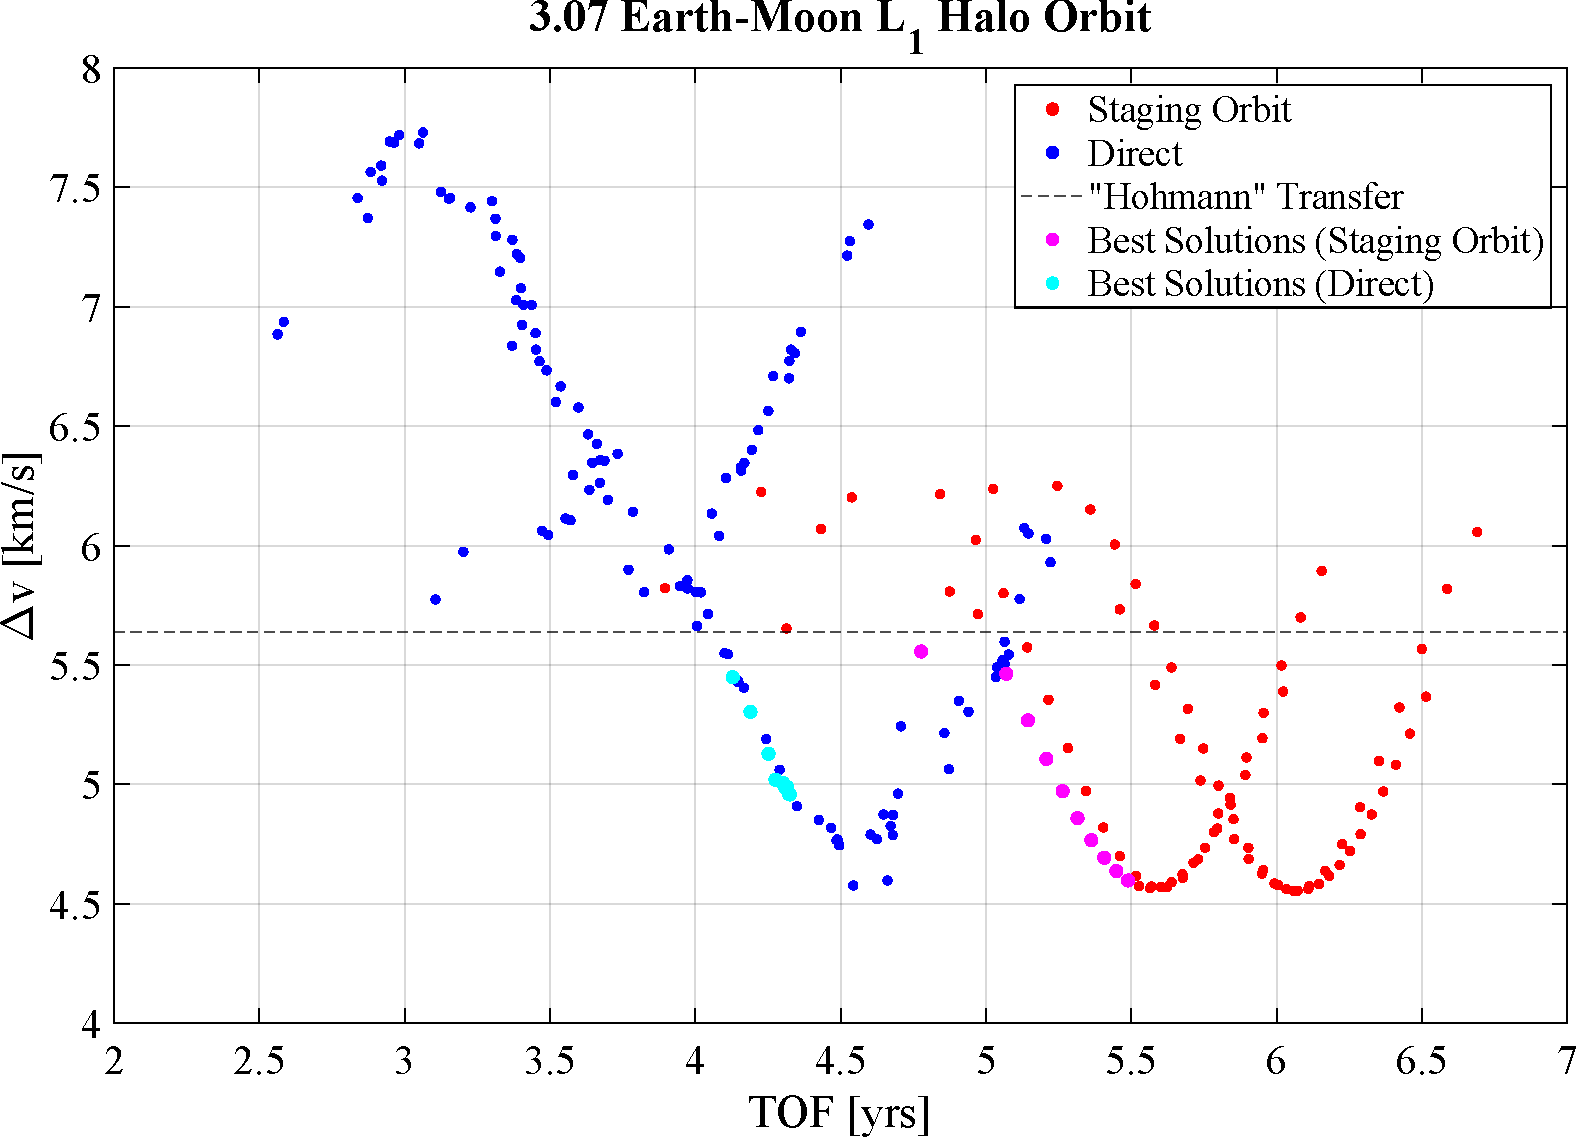
\includegraphics[width=0.75\textwidth]{figures/TradeSpace_L1Halo_3_07.pdf}
    \caption{Transfer tradespace departing from an Earth-Moon $L_{1}$ northern halo orbit ($JC=3.07$).}
    \label{fig:lowDeltav}
\end{figure}

If total TOF and total maneuver $\Delta v$ are considered to have units of years and km/s,
respectively, then these values have similar orders of magnitude for these transfers. Therefore, an
appropriate cost function needs to place weights on the two parameters depending on desired
transfer characteristics that are mission-dependent:
\begin{equation}
    J=\alpha TOF+\beta\Delta v,
    \label{eq:costfunction}
\end{equation}
where $J$ is the cost function value and $\alpha$ and $\beta$ are design variables to adjust the
cost function. $\alpha$ and $\beta$ can be adjusted to put higher priority on TOF or $\Delta v$,
depending on the particular application. This investigation uses $\alpha=5$ and $\beta=2$ to
prioritize lower TOF while still looking for decreased maneuver costs. This cost function is
applied to the transfers in the tradespace that are below the "Hohmann" transfer $\Delta v$
baseline, and the ten transfers from each transfer category that have the lowest $J$-value are
determined to be the best transfers for this application. For the case of the $L_{1}$ halo with
$JC=3.07$ in \cref{fig:lowDeltav}, these are the cyan ("direct") and magenta ("staging") points.

\subsection{Comparison of Selected Transfers}
In \cref{fig:lowDeltav}, among the transfers selected using the cost function, the "direct" options
still have lower times-of-flight, while the transfers with staging orbits achieve lower $\Delta v$
costs. This contrasts with the earlier example from \cref{fig:tradespace}, now shown with the best
solutions from the cost function in \cref{fig:lowBoth}, where the "direct" options have both lower
times-of-flight and maneuver costs. 

\begin{figure}[ht]
    \centering
    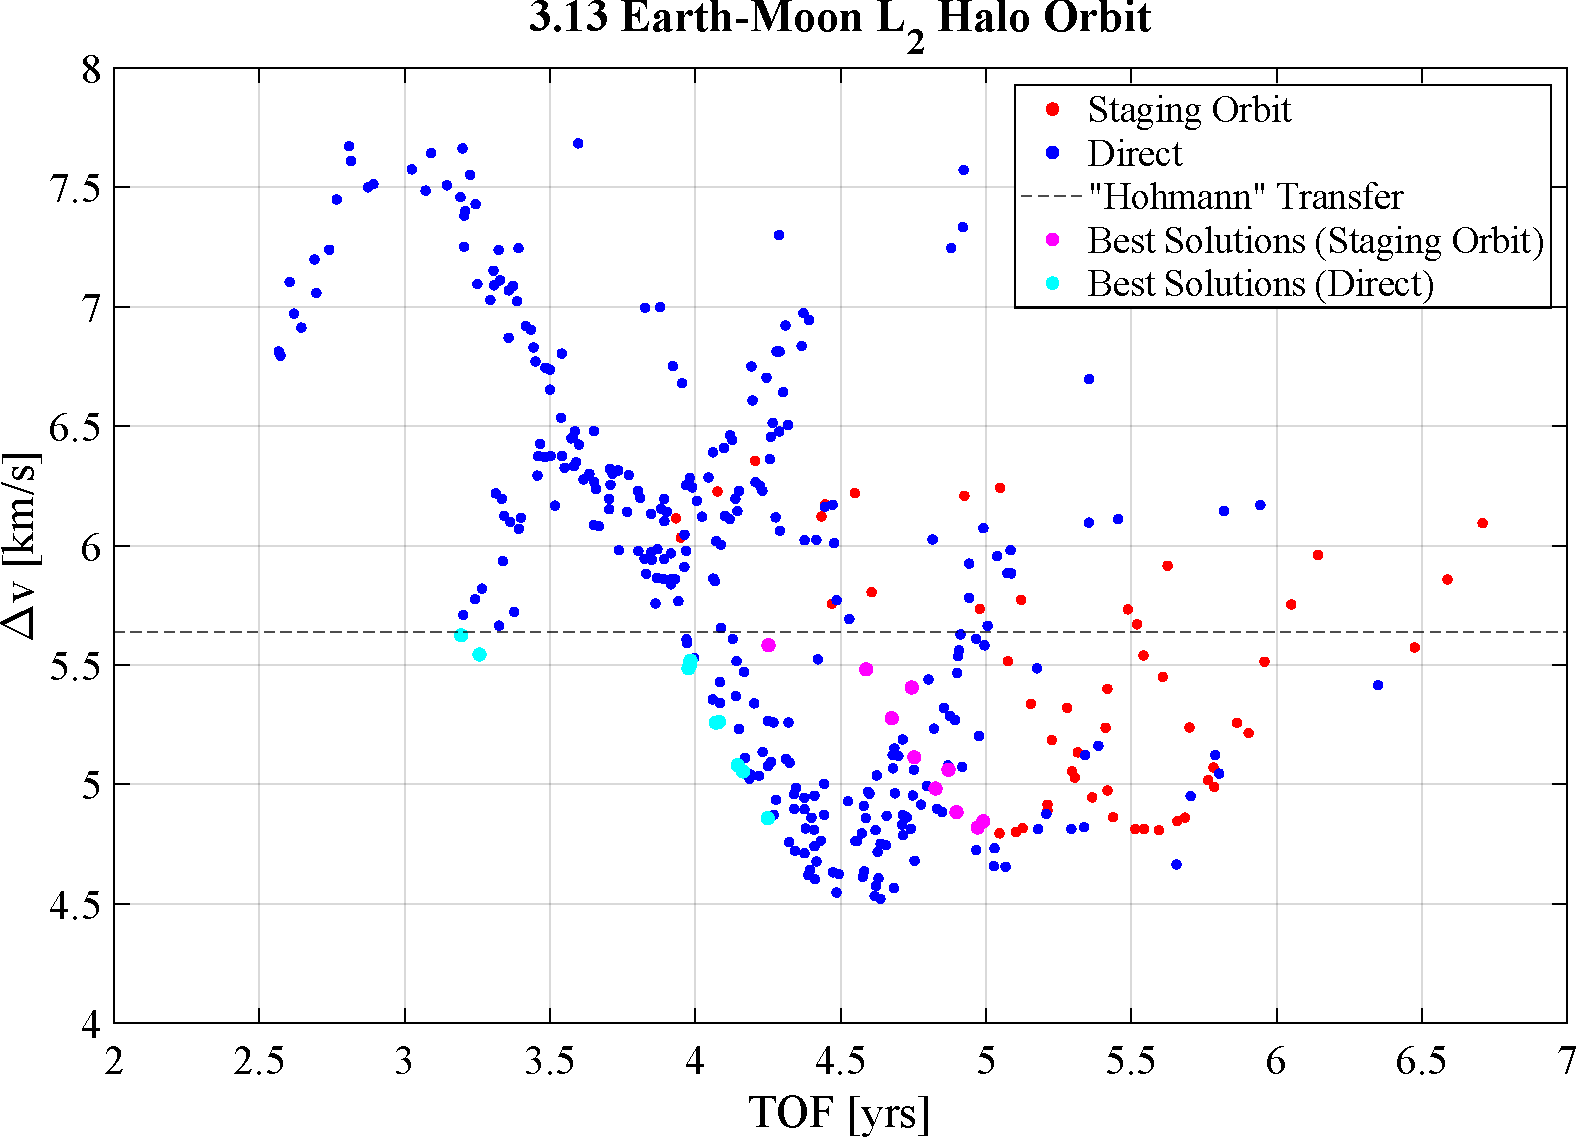
\includegraphics[width=0.75\textwidth]{figures/TradeSpace_L2Halo_3_13.pdf}
    \caption{Transfer tradespace departing from an Earth-Moon $L_{2}$ northern halo orbit ($JC=3.13$).}
    \label{fig:lowBoth}
\end{figure}
